% !TEX TS-program = xelatex
% !TEX encoding = UTF-8 Unicode

% Tennessee Technological University
% ME4140 - Fall 2016 - Fall 2017 - ? - Fall 2019 - Fall 2020 - Fall 2021
% Tristan Hill - August 08, 2020 - August 22, 2021
% Module 1 - ROS Overview

\documentclass[fleqn]{beamer} % for presentation (has nav buttons at bottom)

% custom preamble
\usepackage{/home/thill/Documents/lectures/ros_workshop/ros_lecture}

\newcommand{\MNUM}{1\hspace{2mm}} % Module number
\newcommand{\TNUM}{1\hspace{2mm}} % Topic number 
\newcommand{\moduletitle}{ROS Overview} % Titles and Stuff
\newcommand{\lecturetitle}{Lecture \MNUM - \moduletitle} 

\newcommand{\sectiontitleI}{What is ROS?} % More Titles and Stuff
\newcommand{\sectiontitleII}{Benefits of ROS}
\newcommand{\sectiontitleIII}{How does ROS work?}
\newcommand{\sectiontitleIV}{Supported Hardware and Software}
\newcommand{\sectiontitleV}{Tutorial 1 - Virtualize Ubuntu}

\author{ME4140 - ROS Workshop}
\title{\GD Module \MNUM - \moduletitle}
\date{Mechanical Engineering\vspc Tennessee Technological University}

\begin{document}

\lstset{language=MATLAB,basicstyle=\ttfamily\small,showstringspaces=false}

\frame{\titlepage \center\begin{framed}\Large \textbf{\lecturetitle}\end{framed} \vspace{5mm}}

% Section 0 - Outline
\frame{
	
	\large \textbf{\lecturetitle} \vspace{3mm}\\
	
	\begin{itemize}
	
		\item \hyperlink{sectionI}{\color{black}\sectiontitleI}	\vspace{3mm} % Section I
		\item \hyperlink{sectionII}{\color{black}\sectiontitleII}	\vspace{3mm} % Section II
		\item \hyperlink{sectionIII}{\color{black}\sectiontitleIII}	\vspace{3mm} %Section III
		\item \hyperlink{sectionIV}{\color{black}\sectiontitleIV}	\vspace{3mm} %Section IV
		\item \hyperlink{sectionV}{\color{black}\sectiontitleV} %Section IV	
	
	\end{itemize}

}

% Section I
\section{\sectiontitleI}

	% Section I - Frame I
	\begin{frame}[label=sectionI] \small
		\frametitle{\sectiontitleI}
		
			\begin{itemize}
		\item {\it The Robot Operating System (ROS) is a flexible framework for writing robot software. It is a collection of tools, libraries, and conventions that aim to simplify the task of creating complex and robust robot behavior across a wide variety of robotic platforms.} - \href{http://www.ros.org/about-ros/}{ROS WIKI}  \vspc
        \item Open Source (Creative Commons) Software  Framework for Robotics Development \vspc
        \item not what you may think when you hear {\it operating system}            
            \end{itemize}
	\end{frame}

	% Section I - Frame II
	\begin{frame} \small
		\frametitle{\sectiontitleI}
Where did ROS come from?
            \begin{itemize}
                \item Developed at Stanford (mid 2000s)
                \item Continued by Willow Garage (2007)
                \end{itemize} 
                Where is ROS now?        
            
                \begin{itemize}
                \item Maintained by an international community of developers (present)
                \item {\it The ROS ecosystem now consists of tens of thousands of users worldwide, working in domains ranging from tabletop hobby projects to large industrial automation systems.} - \href{http://www.ros.org/history/}{ROS WIKI}
                \item We are going to use ROS-Melodic (\href{http://wiki.ros.org/Distributions}{timeline})
            \end{itemize} 

	\end{frame}
	
	
% Section II
\section{\sectiontitleII}	

	% Section II - Frame I
	\begin{frame}[label=sectionI] \small
		\frametitle{\sectiontitleII}

		ROS allows us to build upon the knowledge and capabilities of the current state of robotics technology and theory. \vspc

            \begin{itemize}
                \item Hardware/Software Compatibility   
				\item Pre-Compiled Algorithms for Robotics              
                \item Multi-threading, Parallel Processing, Distributed Computing  
                
                \item Open Source Community (\href{https://creativecommons.org/licenses/by/3.0/us/}{Creative Commons})    
                %\item High Level Robotics Development                   
            \end{itemize}    

		\end{frame}

	% Section II - Frame II
	\begin{frame} \small
		\frametitle{\sectiontitleII}
		     Who is using ROS? \vspc
             \begin{itemize}
                \item Researchers  
                \item Students    
                \item Hobbyists
                \item Industry - {\it start ups} and {\it big business (?)} \vspace{5mm}                  
            \end{itemize} 
            
            Who can use ROS? \hspace{10mm} You!
	\end{frame}
		

	% Section III - Frame I
	\begin{frame} \small
		\frametitle{\sectiontitleII}
		\underline{Thought exercise:} Think about designing a robot to move boxes from one location to another in a large room.  
		\begin{itemize}
		\item Where do you begin?  
		\item What does the robot look like?
		\item What major elements or components are required for the robot? \vspace{20mm}
		\end{itemize}
	\end{frame}

% Section III
\section{\sectiontitleIII}	
	% Section IV - Frame I
	\begin{frame}[label=sectionIII] \small
		\frametitle{\sectiontitleIII}

               ROS is organized in a system of connected {\it nodes} which each node represents a different element or component in a robotic system.
                   
                   \begin{itemize}
                        \item Laser
                        \item Drive Kinematics
                        \item Navigation
                        \item Manipulator
                        \item etc.
                    \end{itemize}
	\end{frame}  
	
\section{\sectiontitleIV}	
	% Section IV - Frame I
	    \begin{frame}[label=sectionIV] \small
		\frametitle{\sectiontitleIV}    
                Each node can have corresponding source code, executables, data files, and more. Different software languages are available.
                \begin{itemize}
                \item C++ (instructor support in ME4140)
                \item Python (you are on your own)
                \item {\it markup languages} such as XML and YAML (we may use some)\\
                 \end{itemize}
				
				Pre-built software is avaiable for interfacing with different Robots, sensors, actuators, and other components. Also, ROS can run on small board computers with limited resources. 
				
				\begin{itemize}
				\item Robots! (Adept, Clearpath, UR) 
				\item LIDAR (SICK, RPLidar, etc.) and Cameras (webcam, Kinect, Opti-track)

				\item Motor Drivers (Roboteq, ROSARIA) 
				\end{itemize}

		\end{frame}
		

%            \textbf{ Videos:} \\\\
%       \href{https://youtu.be/wXPLH_2IRVw}{Turtlebot}\\\\
%                \href{https://www.dropbox.com/s/adpg9v3lvfltd92/lx_demo_cut_07_07_2020.mp4?dl=0}{Pinoeer LX}\\\\
%
%                \href{https://youtu.be/lcICvz5jMHw}{Aubo Arm}\\
\section{\sectiontitleV}	
	% Section V - Frame I
	           \begin{frame}[label=sectionV] \small
		\frametitle{\sectiontitleV}    
	
 \setbeamertemplate{itemize items}[triangle]
                \begin{itemize}

					\item {\bf Overview:} ROS runs on Linux! Your first exercise is to setup your computer so that you can begin learning ROS. 		

					\item {\bf Assignment:} Complete the tutorial \href{https://github.com/thillRobot/ros\textunderscore workshop/blob/master/module1/tutorial1\textunderscore virtualize\textunderscore ubuntu/tutorial1\textunderscore virtualize\textunderscore ubuntu.md}{tutorial1\textunderscore virtualize\textunderscore ubuntu}. After completion your new system should be able to access the internet.
                    
                    \item {\bf Deliverable:} Write a one to two paragraph summary of what you accomplished and what you struggled with the most. Include an image of your Ubuntu desktop. 
    
                    \item {\bf Next Week:} After completion of Module 1, you will be ready to install the ROS Melodic software package in Ubuntu 18.04. This is described in detail in Module 2. \vspc
                    
    
                \end{itemize}
		\end{frame}

\end{document}



%%            \item [How to get Started!]: There are several ways to get started but it is recommended that you use Ubuntu 16 LTS. ROS is also available for Ubuntu 18 LTS. There has also been talk of ROS on windows. 
%%                \begin{enumerate}
%%                    \item Install Ubuntu - 3 options
%%                        \begin{enumerate}
%%                            \item Virtualize Ubuntu with {\it Virtual Box}
%%                            \item Install Ubuntu permanently on your machine {\it True Boot}
%%                            \item Run Ubuntu temporarily on your machine {\it wubi.exe boot}        
%%                        \end{enumerate}
%%                    
%%                    \item Install ROS Indigo
%%                        \begin{enumerate}
%%                            \item before you change your linux system it is a good idea to back it up!
%%                            \item make sure your system can connect to the internet
%%                            \item check that your system can successfully update (not upgrade OS)
%%                            \item in a terminal \$sudo apt-get check , you  will be prompted for the administrator password and if you do not see any errors you are ready to go!      
%%                        \end{enumerate}
%%                    
%%                \end{enumerate}


%\begin{document}
%
%\thispagestyle{plain}
%
%\begin{center}
%    {\bf \Large ROS - The Robotic Operating System} \vspace{3mm} \\
%   {\bf \large ME 4140 - Introduction to Robotics - Fall 2020} \\
%\end{center}
%
%\Large
%\begin{description}
%
%    	\item[What is ROS?]: 
%            \begin{enumerate}
%		\item {\it The Robot Operating System (ROS) is a flexible framework for writing robot software. It is a collection of tools, libraries, and conventions that aim to simplify the task of creating complex and robust robot behavior across a wide variety of robotic platforms.} - \href{http://www.ros.org/about-ros/}{ROS}       
%                 \item Software Framework for Robotics Development
%                \item {\it not} what you may think when you hear {\it operating system}                    
%            \end{enumerate}
%      
%        \item[What are the benefits of using ROS?]: 
%            \begin{enumerate}
%                \item Hardware/Software Compatibility   
%                \item Multi-threading, Parallel Processing, Distributed Computing  
%                \item Open Source Community (BSD)    
%                \item High Level Robotics Development                   
%            \end{enumerate}    
%            
%%        \item[Who is using ROS?]:
%%             \begin{enumerate}
%%                \item Researchers  
%%                \item Students    
%%                \item Industry - {\it start ups} and {\it big business (?)}                  
%%            \end{enumerate} 
%
%        \item[Where did ROS come from?]:
%            \begin{enumerate}
%                \item Originally developed at Stanford (mid 2000s)
%                \item Continued by Willow Garage (2007)
%                \item Maintained by an international community of open source developers (present)
%                \item {\it The ROS ecosystem now consists of tens of thousands of users worldwide, working in domains ranging from tabletop hobby projects to large industrial automation systems.} - \href{http://www.ros.org/history/}{ROS}
%            \end{enumerate} 
%
%            \newpage
%            
%            \item [How Does it Work?]:
%            \begin{enumerate}
%                \item ROS is based on a system of connected {\it nodes} 
%                \item Each node represents a different element in the robotic system
%                   
%                   \begin{itemize}
%                        \item Laser
%                        \item Drive Kinematics
%                        \item Navigation
%                        \item Manipulator
%                        \item etc.
%                    \end{itemize}
%                \vspace{15mm}
%                \item Each node can have corresponding source code, executables, and data files.\\
%\item Software Languages
%                \begin{itemize}
%                \item C++ 
%                \item Python
%                \item {\it markup languages} such as XML and YAML\\
%                 \end{itemize}
%                 
%                \item Nodes communicate or share information in  different ways. 
%                 \begin{itemize}
%                        \item Topics - {\it publish} and {\it subscribe} to specific information.
%                        \item Parameter Server - Static Data
%                        \item Services - RPC - Single Request \\\\
%                    \end{itemize} 
%                
%                \item The parallel processing and message passing is handled by ROS. Distributed computing is supported for off board computing and multi-robot applications.
%            \end{enumerate}    
%         
%         \newpage
%         \item [Supprted Robots]:\\
%                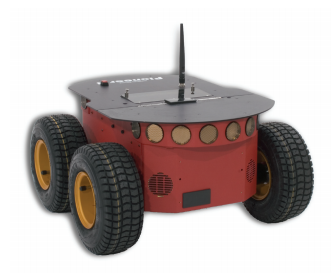
\includegraphics[scale=1]{p3at.PNG}
%            
%
%                
%            \newpage
%            \textbf{ Videos:} \\\\
%       \href{https://youtu.be/wXPLH_2IRVw}{Turtlebot}\\\\
%                \href{https://www.dropbox.com/s/adpg9v3lvfltd92/lx_demo_cut_07_07_2020.mp4?dl=0}{Pinoeer LX}\\\\
%
%                \href{https://youtu.be/lcICvz5jMHw}{Aubo Arm}\\
%
%%            \item [How to get Started!]: There are several ways to get started but it is recommended that you use Ubuntu 16 LTS. ROS is also available for Ubuntu 18 LTS. There has also been talk of ROS on windows. 
%%                \begin{enumerate}
%%                    \item Install Ubuntu - 3 options
%%                        \begin{enumerate}
%%                            \item Virtualize Ubuntu with {\it Virtual Box}
%%                            \item Install Ubuntu permanently on your machine {\it True Boot}
%%                            \item Run Ubuntu temporarily on your machine {\it wubi.exe boot}        
%%                        \end{enumerate}
%%                    
%%                    \item Install ROS Indigo
%%                        \begin{enumerate}
%%                            \item before you change your linux system it is a good idea to back it up!
%%                            \item make sure your system can connect to the internet
%%                            \item check that your system can successfully update (not upgrade OS)
%%                            \item in a terminal \$sudo apt-get check , you  will be prompted for the administrator password and if you do not see any errors you are ready to go!      
%%                        \end{enumerate}
%%                    
%%                \end{enumerate}
%                    
%         
%            
%\end{description}
%
%
%\end{document}
%
